\documentclass[11pt]{article}
%Gummi|065|=)
\title{\textbf{CV Homework 3}}
\author{Eric Feuvrier Danziger\\
		}
\date{}
\usepackage{graphicx}
\usepackage{float}
\usepackage{amsmath}
\begin{document}

\maketitle

\section*{1.1 Planar Homography}
The plane $\Pi$ constrains the value of P to be 2 dimensional. If you set the dimension normal to the plane to be z, then the point P can be described only using x and y. 

The existing projection matrix M moves from the world to the image coordinates. 

The existing M $ \begin{bmatrix}
m11 & m12 & m13 & m14\\
m21 & m22 & m23 & m24 \\
m31 & m32 & m33 & m34\\ \end{bmatrix} $
can be rewritten as a 3x3 matrix when you drop out the third dimension. 
\\
$M_1 * \begin{array} {c}
x \\
y \\
z \\
1 \end{array} $ can be rewritten as 
$ M_{1\Pi} * \begin{array} {c}
x \\
y \\
1 \end{array}$ where $M_{1\Pi}$ is 3x3. 
The p and q equations can be rewritten as \\
$p = M_{1\Pi} P_{\Pi} \\
q = M_{2\Pi} P_{\Pi} \\ 
P = M_{2\Pi}^{-1}q \\
p = M_{1\Pi}M_{2\Pi}^{-1}q$
You can then say that $H=M_{1\Pi}M_{2\Pi}^{-1}$

\section*{1.2 Homography by Rotation}
$p=Hq$\\
$p=H(K_2[R\ 0]P) = K_1[I\ 0]P$\\
$K_2[R\ 0]P$ can be rewritten as $K_2R\hat{P}$ because the fourth column is a zero vector. This means that the scale factor drops off the P value, leaving only a 3x1 xyz vector. 
This also leads to $K_1[I 0]P$ being set to $K_1[I]\hat{P}$
With the new 3x3 values for the projection and 3x1 values for the point $\hat{P}$ you can rewrite \\
$p = K_1I\hat{P}$ as \\
$p = K_1I[K_2R]^{-1}q$\\
$p = K_1R^{-1}K_2^{-1}q$\\
$p = K_1R^TK_2^{-1}q$\\
with $H = K_1R^TK_2^{-1}$

\section*{1.3 Sufficiency}
The planar homography is not sufficient because it assumes either 0 translation of the camera or that the points are on a plane $\Pi$. Since the world is three dimensional and not planar, all the points in the world $P$ will not be on the same plane. An example would be points that can be occluded from view at different vantage points by the 3D structure of an object. 

\section*{1.4 Deriving H}
\subsection*{1.4.a}
$\begin{bmatrix}
x\\
y\\
1\\ \end{bmatrix} = \begin{bmatrix}
h11 & h12 & h13\\
h21 & h22 & h23\\
h31 & h32 & h33\\ \end{bmatrix} 
\begin{bmatrix}
u\\
v\\
1\\ \end{bmatrix} \\
x_i = H_{11}u_i + H_{12}v_i + H_{13}\\
y_i = H_{21}u_i + H_{22}v_i + H_{23}\\
1 = H_{31}u_i + H_{32}v_i + H_{33}\\
$ Dividing the first and second equations by the first you get \\
$
x_i = \frac{H_{11}u_i + H_{12}v_i + H_{13}}{H_{31}u_i + H_{32}v_i + H_{33}}\\
y_i =\frac{H_{21}u_i + H_{22}v_i + H_{23}}{H_{31}u_i + H_{32}v_i + H_{33}}\\
x_i(H_{31}u_i + H_{32}v_i + H_{33}) = H_{11}u_i + H_{12}v_i + H_{13}\\
y_i(H_{31}u_i + H_{32}v_i + H_{33}) = H_{21}u_i + H_{22}v_i + H_{23}\\
x_i(H_{31}u_i + H_{32}v_i + H_{33}) - (H_{11}u_i + H_{12}v_i + H_{13})= 0\\
y_i(H_{31}u_i + H_{32}v_i + H_{33}) - (H_{21}u_i + H_{22}v_i + H_{23}) = 0
$ These are the 2 equations that make up the A matrix. This is why there are 2N rows in A. 
$a_x = 
\begin{bmatrix}
-u_i & -v_i & -1 & 0 & 0 & 0 & x_iu_i & x_iv_i & x_i\\ \end{bmatrix}\\
a_y = 
\begin{bmatrix}
0 & 0 & 0 & -u_i & -v_i & -1 &  y_iu_i & y_iv_i & y_i\\ \end{bmatrix}\\
A =
\begin{bmatrix}
a_{1x}\\
a_{1y}\\
.\\
.\\
.\\
a_{Nx}\\
a_{Ny}\\
 \end{bmatrix}
$
\subsection*{1.4.b}
There are 9 elements in h.\\
$h = \begin{bmatrix}
h11\\
h12\\
h13\\
h21\\
h22\\
h23\\
h31\\
h32\\ 
h33\\ \end{bmatrix} 
$
\subsection*{1.4.c}
A is 2Nx9
\subsection*{1.4.d}
There are 8 degrees of freedom in H because of the scale factor. Each correspondance gives us 4 variables (x,y,u,v) and 2 equations. 
\subsection*{1.4.e}
The sum squared error of $Ah = 0$ can be written\\
$f(h) = \frac{1}{2}(Ah - 0)^T(Ah-0)$\\
$f(h) = \frac{1}{2}(Ah)^T(Ah)$\\
$f(h) = \frac{1}{2}h^TA^TAh$\\
taking the derivative of f with respect to h and setting it to zero\\
$\frac{d}{dh}f = 0 = \frac{1}{2}(A^TA + (A^TA)^T)h$\\
$ = A^TAh$\\
Looking at the eigen-decomposition of $A^TA$, we see that h should equal the eigenvector of $A^TA$ that is zero or closest to zero. This is the smallest column of V from SVD. \\
(From \textit{Homography Estimation} by David Kreigman)
\\
\\
\subsection*{3.1.b}

\begin{figure}[H]
\centering
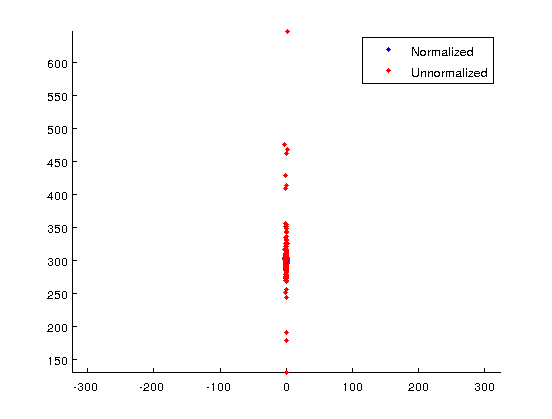
\includegraphics[width=90mm]{results/q3_1.png}
\caption{Normalized vs Unnormalized }
\end{figure}
\begin{figure}[H]
\centering
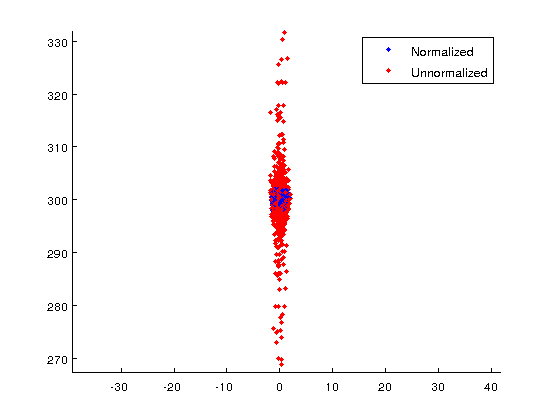
\includegraphics[width=90mm]{results/q3_1zoomed.png}
\caption{Normalized vs Unnormalized Zoomed In }
\end{figure}

\subsection*{3.1.c}
Running the ratio test once I get a value of 47, meaning the unnormalized version has 47 times the standard deviation of the normalized. \\
\subsection*{3.1.d}
Running it a few times, I get values between 20 and 60, meaning that the normalized version is consistently better. Visually the cluster of points is similar every time to the figures above, a nice clustered ball for the normalized points and a long trailing set for the unnormalized. This tells you that the normalized has a better result, with lower error on average, every time. 
\subsection*{4.1}
\begin{figure}[H]
\centering
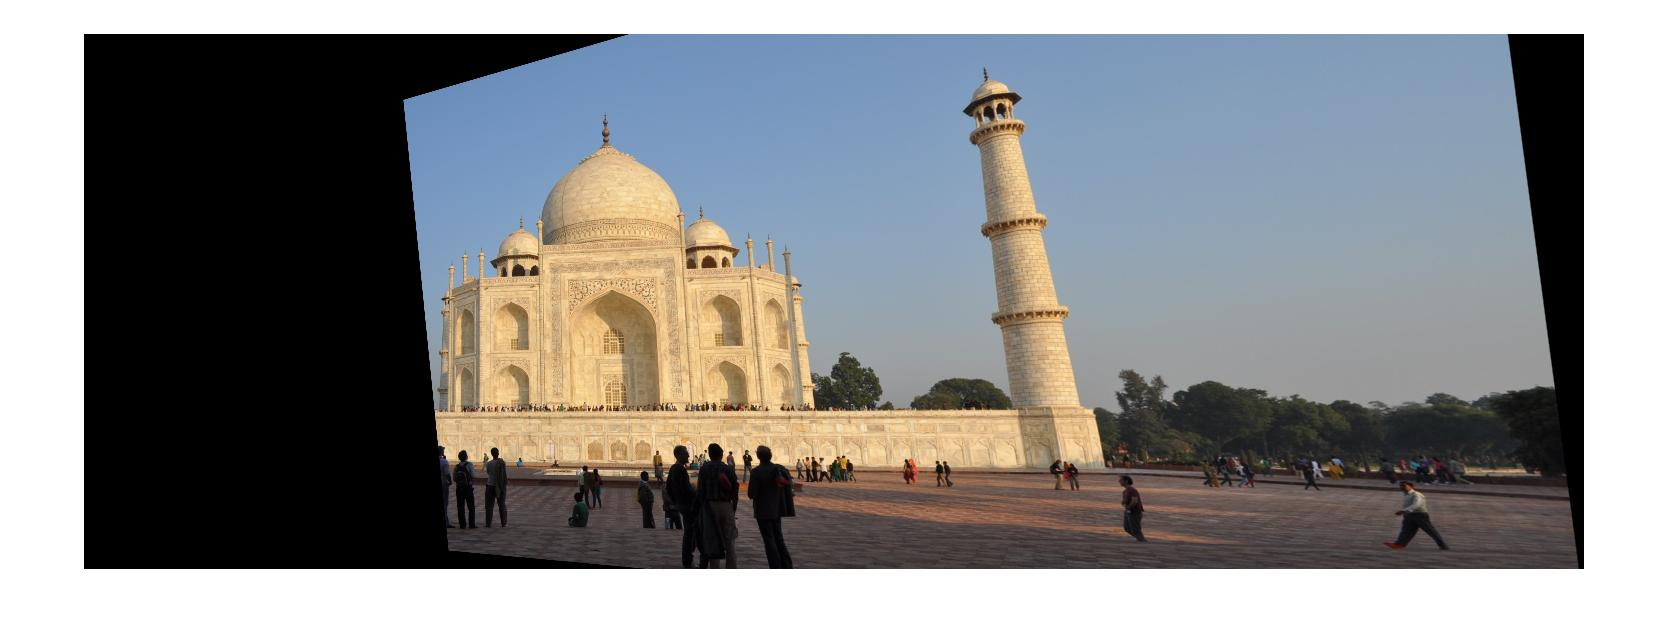
\includegraphics[width=90mm]{results/q4_1.jpg}
\caption{Warped Image }
\end{figure}
\begin{figure}[H]
\centering
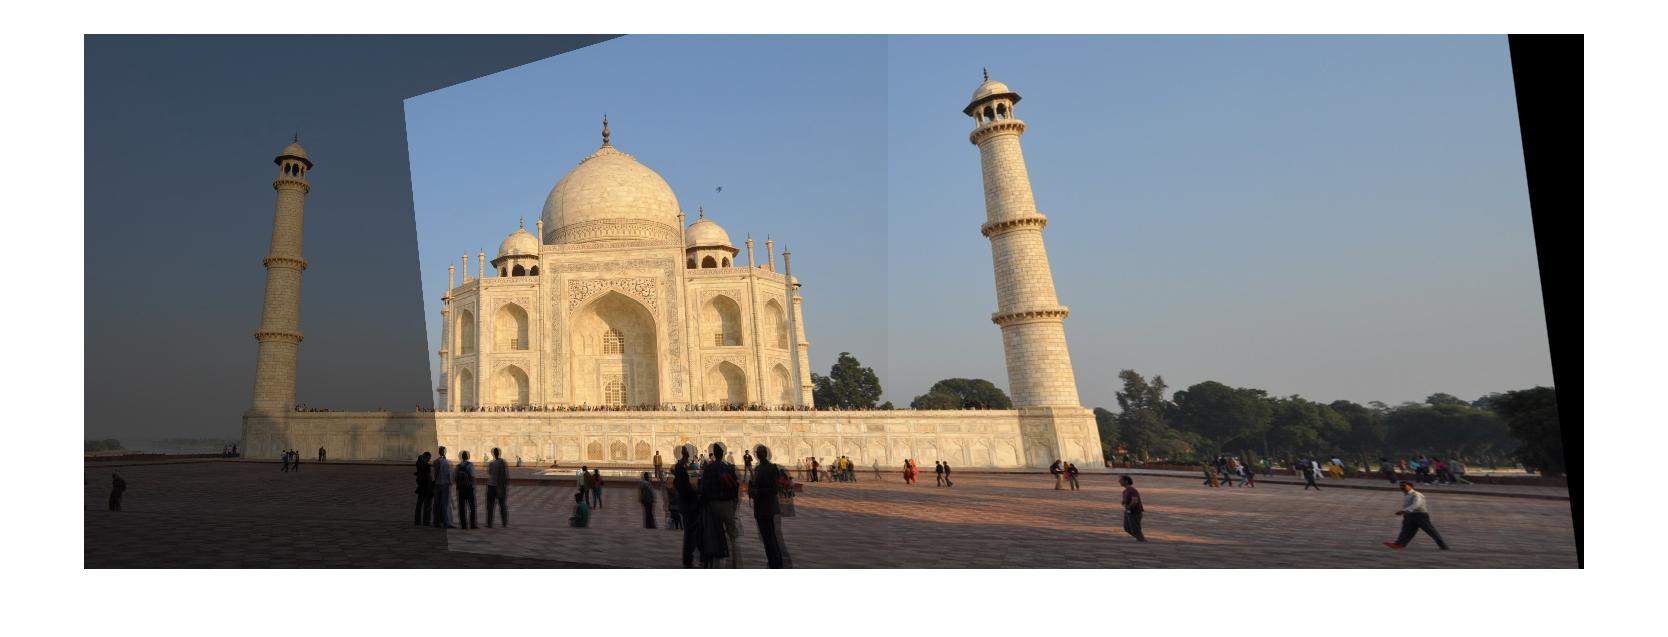
\includegraphics[width=90mm]{results/q4_1_pan.jpg}
\caption{Stitched Image }
\end{figure}
\subsection*{4.2}
\begin{figure}[H]
\centering
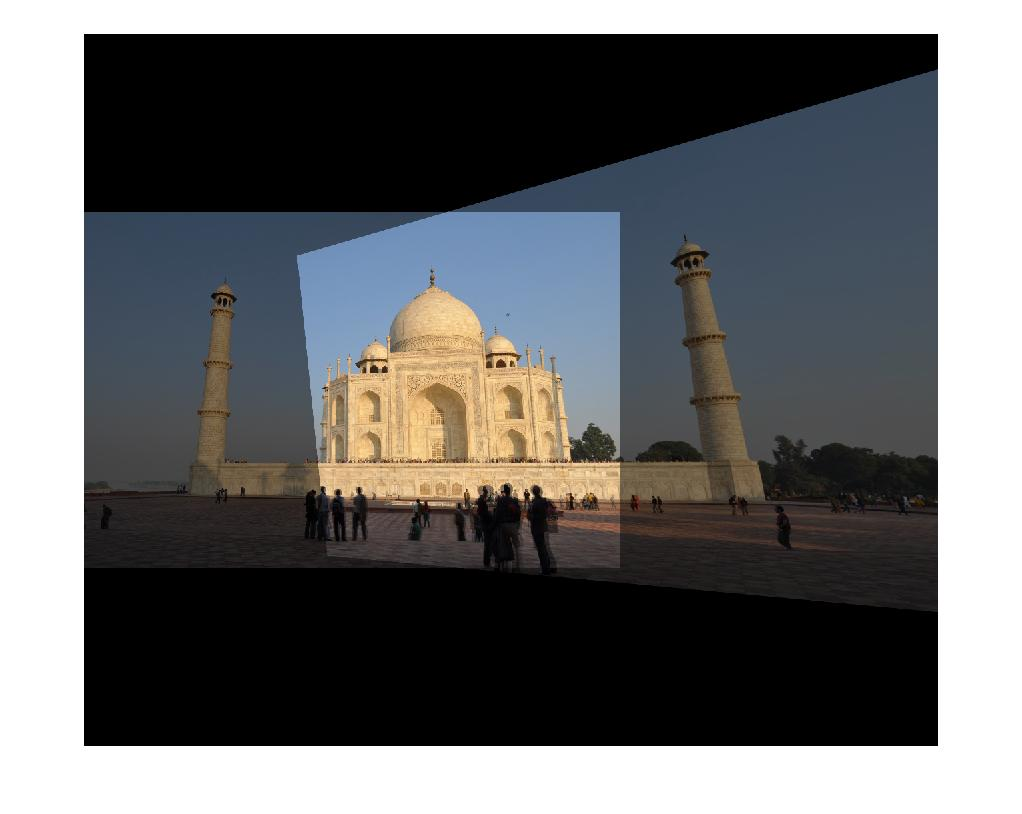
\includegraphics[width=90mm]{results/q4_2_pan.jpg}
\caption{Warped and Centered Image}
\end{figure}

\subsection*{5.2}
\begin{figure}[H]
\centering
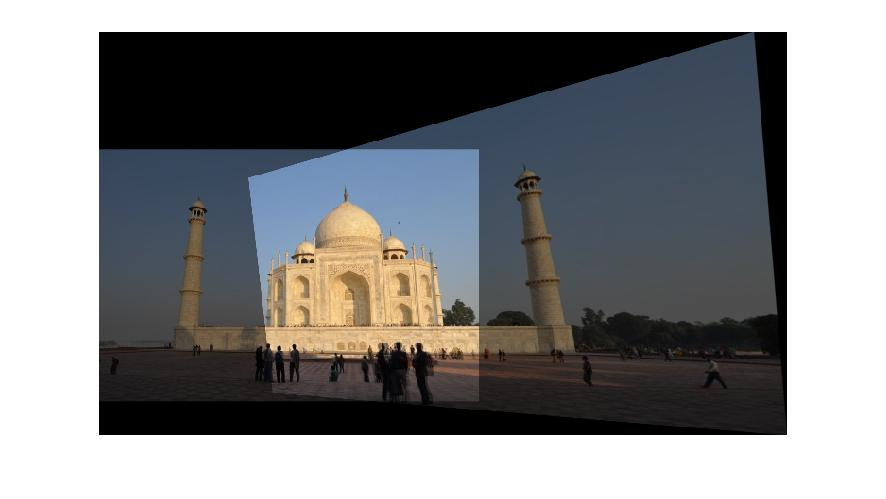
\includegraphics[width=90mm]{results/q5_2.jpg}
\caption{Warped and Centered Image}
\end{figure}
\subsection*{Extra Credit}
This was taken outside Newell Simon Hall
\begin{figure}[H]
\centering
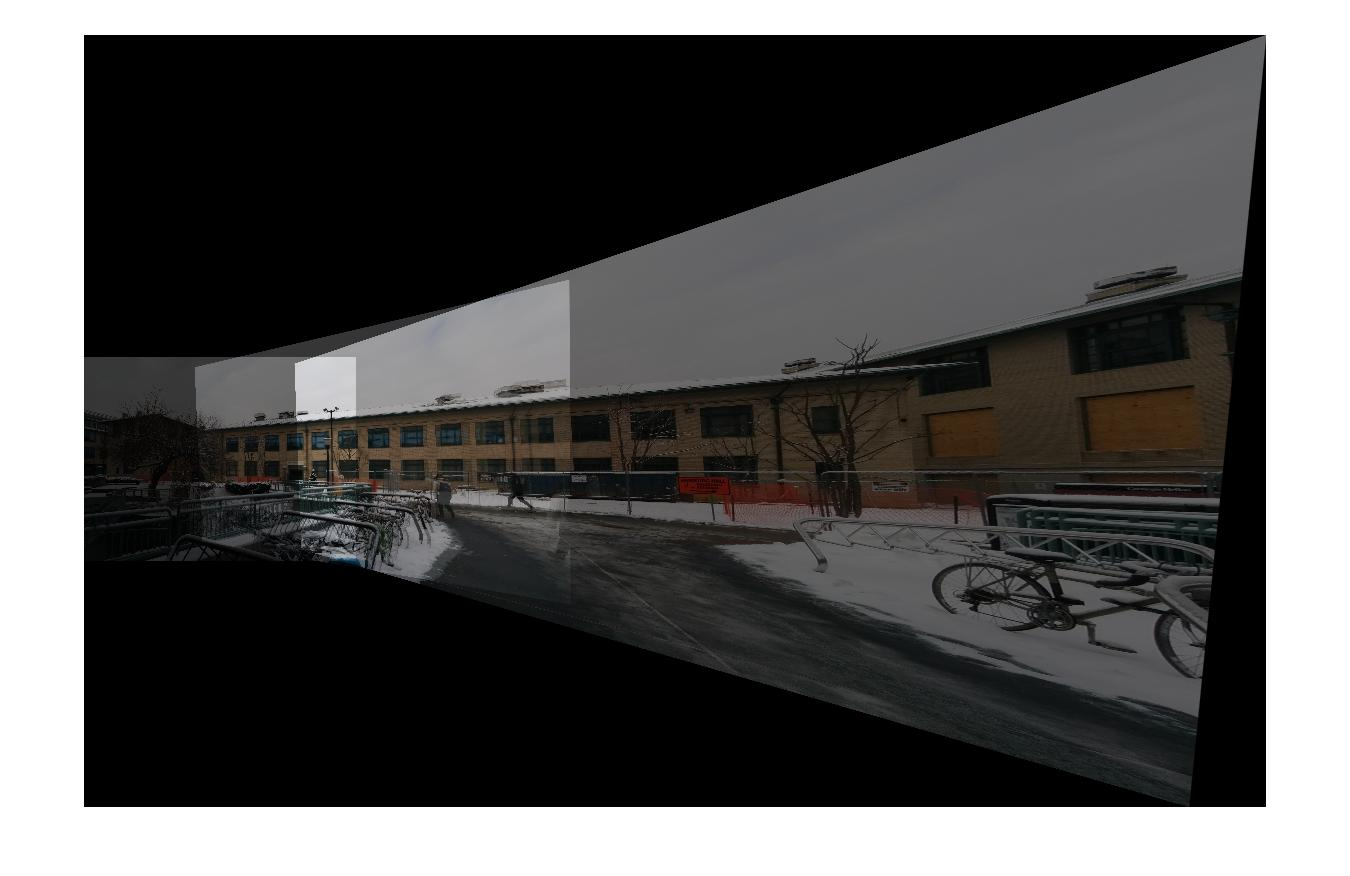
\includegraphics[width=150mm]{results/ec_pan.jpg}
\caption{Warped and Centered Image}
\end{figure}

\end{document}
